\documentclass[a4paper, 12pt]{article}
\usepackage[utf8]{inputenc}
\usepackage{amsmath}
\usepackage{amsfonts}
\usepackage{graphicx}
\usepackage{hyperref}
%\usepackage{tikz}
%\usetikzlibrary{positioning}

\title{Apprentissage par Renforcement pour le Contrôle d'un Drone}
\author{Inès Hafassa-Maïza, Hugo Laval}
\date{\today}

\begin{document}

\maketitle

\section{Introduction}
Ce rapport décrit l'utilisation de l'apprentissage par renforcement pour contrôler un drone dans un environnement 3D avec des obstacles. Le but est de permettre au drone de naviguer de manière autonome vers une destination tout en évitant les obstacles.

\section{Modélisation}
Nous avons choisi la modélisation suivante pour le problème. Notre drone évolue dans un cube de côté 10. Dans ce cube, se trouvent des obstacles sphériques de taille variable. Nous générons une position initiale et une destination, toutes deux de manière aléatoire selon une loi uniforme et nous nous assurons que ni le point de départ, ni la destination ne se trouvent à l'intérieur d'un obstacle.

Notre drone est modélisé par une sphère de volume $\epsilon$, si bien que si la position du drone (matérialisée par son centre) atteint la destination à moins de $\epsilon$ près, c'est-à-dire si la norme L2 pour cette distance est inférieure à $\epsilon$, alors on considère que le drone a livré son colis avec succès. De même, si le drone passe à moins de $\epsilon$ d'un obstacle, il échoue.

Afin de détecter les obstacles, le drone possède des radars omnidirectionnels lui permettant de détecter des obstacles dans un rayon de 10 unités pour la norme L2 de $\mathbb{R}^3$. Le drone peut progresser en faisant des pas de distance fixe. À chaque étape, le drone calcule la direction pour atteindre la cible en ligne droite et recherche la présence d'obstacles dans cette direction (dans la limite de son rayon de détection). Si un obstacle est détecté, notre drone choisira sa nouvelle trajectoire en utilisant un algorithme d'apprentissage par renforcement appelé Actor-Critic que nous allons détailler.

\subsection{Génération des Obstacles}
Les obstacles dans l'environnement sont générés de manière aléatoire en suivant des lois de probabilités spécifiques :
\begin{itemize}
    \item \textbf{Nombre d'obstacles} : Le nombre d'obstacles est tiré aléatoirement selon une loi uniforme discrète entre 0 et 10.
    \item \textbf{Position des obstacles} : Les centres des obstacles sont générés selon une loi uniforme continue dans le cube de côté 10. Chaque coordonnée $(x, y, z)$ du centre est tirée indépendamment selon une loi uniforme $U(0, 10)$.
    \item \textbf{Rayon des obstacles} : Les rayons des obstacles sont tirés selon une loi uniforme continue entre 0.5 et 2.5 (soit $\frac{10}{4}$).
\end{itemize}

La génération des obstacles est implémentée comme suit :
\begin{verbatim}
def generate_obstacles(self):
    obstacles = []
    num_obstacles = np.random.randint(0, 10)
    for _ in range(num_obstacles):
        # Random position for the center of the sphere
        center = np.random.uniform(0, self.size, size=3)
        # Random radius for the sphere
        radius = np.random.uniform(0.5, self.size / 4)
        obstacles.append((center, radius))
    return obstacles
\end{verbatim}

Cette méthode assure que les obstacles sont distribués de manière aléatoire dans l'espace de l'environnement, créant ainsi des scénarios variés pour l'apprentissage du drone.

\section{Formulation du Problème}
Le problème est formulé comme un processus de décision markovien (MDP) défini par l'ensemble $(S, A, P, R, \gamma)$ où :
\begin{itemize}
    \item $S$ est l'ensemble des états, représentant la position, la vitesse, la batterie du drone et la destination finale. Plus précisément, $S \subseteq \mathbb{R}^{10}$, où chaque état est un vecteur de dimension 10 comprenant les coordonnées $(x, y, z)$ de la position, les composantes $(Vx, Vy, Vz)$ de la vitesse, le niveau de batterie $B$, et les coordonnées $(x_d, y_d, z_d)$ de la destination.
    \item $A$ est l'ensemble des actions, représentant les accélérations possibles du drone dans les trois directions de l'espace. Plus précisément, $A \subseteq \mathbb{R}^3$, où chaque action est un vecteur de dimension 3 comprenant les composantes $(Ax, Ay, Az)$ de l'accélération.
    \item $P$ est la fonction de transition d'état, définissant la probabilité de passer d'un état à un autre après une action. $P : S \times A \times S \rightarrow [0, 1]$ est une distribution de probabilité sur les états futurs donnée l'état actuel et l'action choisie.
    \item $R$ est la fonction de récompense, définissant la récompense reçue après chaque transition. $R : S \times A \rightarrow \mathbb{R}$ est une fonction qui attribue une valeur réelle à chaque paire état-action, représentant la récompense immédiate obtenue.
    \item $\gamma$ est le facteur de discount, représentant l'importance des récompenses futures. $\gamma \in [0, 1]$ est un scalaire qui pondère les récompenses futures par rapport aux récompenses immédiates.
\end{itemize}

L'objectif est de trouver une politique $\pi(a|s)$ qui maximise la récompense cumulée attendue :
\[
G_t = \mathbb{E} \left[ \sum_{k=0}^{\infty} \gamma^k R_{t+k+1} \mid S_t = s \right]
\]

\section{Modélisation de la Fonction de Récompense et de l'Environnement}
La fonction de récompense est un élément crucial dans l'apprentissage par renforcement, car elle guide l'agent (le drone) vers un comportement optimal. Dans notre implémentation, la fonction de récompense est conçue pour encourager le drone à atteindre sa destination tout en évitant les obstacles. Si le drone atteint sa destination, une récompense élevée de 1000 est attribuée. En revanche, une pénalité sévère de -500 est appliquée en cas de collision avec un obstacle. De plus, pour chaque mouvement, une récompense proportionnelle à la réduction de la distance par rapport à la destination est calculée, incitant le drone à se rapprocher de son objectif. Une pénalité énergétique est également appliquée pour chaque action, proportionnelle à la racine de l'accélération utilisée, afin de simuler la consommation de la batterie.

L'environnement est modélisé comme un cube tridimensionnel de taille fixe (10 unités de côté), rempli d'obstacles générés aléatoirement. La destination est également générée aléatoirement à chaque initialisation de l'environnement. Le drone perçoit son environnement à travers ses états internes, qui incluent sa position, sa vitesse et son niveau de batterie. Ces informations sont encapsulées dans un vecteur d'observation qui est utilisé par le modèle Actor-Critic pour prendre des décisions. Les obstacles sont perçus indirectement par le drone lorsqu'il vérifie les collisions après chaque mouvement. Cette modélisation permet de simuler un environnement réaliste et dynamique pour l'apprentissage du drone.

Les variables d'état du drone sont modélisées comme suit :
\begin{itemize}
    \item $(X)_t, (Y)_t, (Z)_t \in [0, 10]$ représentent les coordonnées de la position du drone à l'instant $t$.
    \item $(Vx)_t, (Vy)_t, (Vz)_t \in \mathbb{R}$ représentent les composantes de la vitesse du drone à l'instant $t$.
    \item $(B)_t \in [0, 10000]$ représente le niveau de batterie du drone à l'instant $t$.
\end{itemize}

Nous définissons également :
\begin{itemize}
    \item $\mathbf{X}_{\text{cible}}$ : le point de livraison.
    \item $\mathcal{O}$ : l'ensemble des obstacles.
\end{itemize}

La fonction de coût $C_t$ à minimiser est définie comme suit :
\[
C_t = -R_t = 
-1000 \cdot \mathbf{1}_{\{\mathbf{X}_t = \mathbf{X}_{\text{cible}}\}} + 500 \cdot \mathbf{1}_{\{\mathbf{X}_t \in \mathcal{O}\}} + 1000 \cdot \mathbf{1}_{\{(B)_t = 0\}} - \alpha \left\| \mathbf{X}_{t+1} - \mathbf{X}_t \right\|_2 + \beta \left\| \mathbf{A}_t \right\|_2
\]
où $\alpha$ et $\beta$ sont des coefficients de pondération pour la distance parcourue et la consommation d'énergie, respectivement, $\mathbf{X}_t = (X_t, Y_t, Z_t)$ représente la position du drone à l'instant $t$, et $\mathbf{A}_t = (Ax_t, Ay_t, Az_t)$ représente les composantes de l'accélération appliquée au drone à l'instant $t$.

\begin{figure}[h]
    \centering
    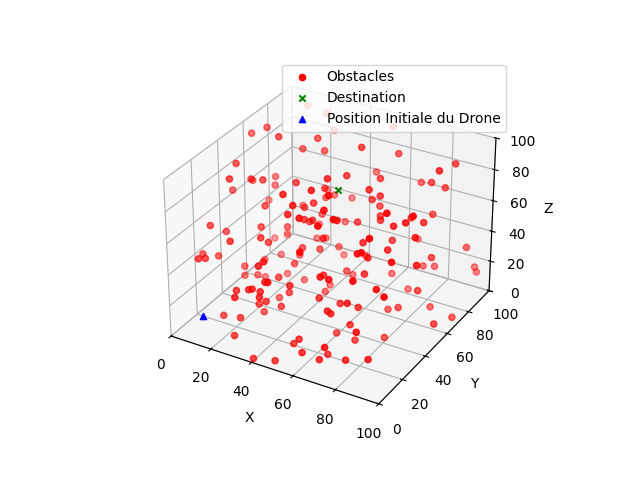
\includegraphics[width=0.8\textwidth]{Figure_1.png}
    \caption{Représentation de l'environnement 3D avec les obstacles et la destination.}
    \label{fig:environment}
\end{figure}

\section{Modèle Actor-Critic}
Le modèle Actor-Critic est utilisé pour résoudre ce problème. Il combine deux réseaux de neurones :
\begin{itemize}
    \item L'actor, qui propose des actions basées sur les états actuels.
    \item Le critic, qui évalue la qualité des actions proposées en estimant la valeur des états.
\end{itemize}

\subsection{Fonctionnement}
Le réseau Actor-Critic fonctionne en deux étapes :
\begin{enumerate}
    \item L'actor prend un état $s$ et propose une action $a$ en suivant une politique $\pi(a|s)$.
    \item Le critic évalue cette action en calculant la valeur de l'état $V(s)$ et l'avantage $A(s, a)$.
\end{enumerate}

\subsection{Fonction Objectif}
L'objectif de l'algorithme Actor-Critic est une combinaison du gradient de politique (pour l'actor) et de la fonction de valeur (pour le critic). La fonction objectif globale est généralement exprimée comme la somme de deux composants :
\begin{itemize}
    \item \textbf{Gradient de Politique (Actor)} :
    \[
    \nabla_\theta J(\theta) \approx \frac{1}{N} \sum_{i=0}^{N} \nabla_\theta \log \pi_\theta(a_i \mid s_i) \cdot A(s_i, a_i)
    \]
    où $J(\theta)$ représente le retour attendu sous la politique paramétrée par $\theta$, $\pi_\theta(a \mid s)$ est la fonction de politique, $N$ est le nombre d'expériences échantillonnées, $A(s, a)$ est la fonction d'avantage représentant l'avantage de prendre l'action $a$ dans l'état $s$, et $i$ représente l'index de l'échantillon.
    \item \textbf{Mise à Jour de la Fonction de Valeur (Critic)} :
    \[
    \nabla_w J(w) \approx \frac{1}{N} \sum_{i=1}^{N} \nabla_w (V_w(s_i) - Q_w(s_i, a_i))^2
    \]
    où $\nabla_w J(w)$ est le gradient de la fonction de perte par rapport aux paramètres du critic $w$, $V_w(s_i)$ est l'estimation du critic de la valeur de l'état $s$ avec le paramètre $w$, et $Q_w(s_i, a_i)$ est l'estimation du critic de la valeur de l'action $a$.
\end{itemize}

\subsection{Fonction d'Avantage}
La fonction d'avantage, $A(s, a)$, mesure l'avantage de prendre l'action $a$ dans l'état $s$ par rapport à la valeur attendue de l'état sous la politique actuelle :
\[
A(s, a) = Q(s, a) - V(s)
\]
où $Q(s, a)$ est la valeur de l'action et $V(s)$ est la valeur de l'état.

\section{Avantages de l'Algorithme Actor-Critic}
L'algorithme Actor-Critic offre plusieurs avantages :
\begin{itemize}
    \item \textbf{Efficacité de l'Échantillon Améliorée} : La nature hybride des algorithmes Actor-Critic conduit souvent à une meilleure efficacité de l'échantillon, nécessitant moins d'interactions avec l'environnement pour atteindre des performances optimales.
    \item \textbf{Convergence Plus Rapide} : La capacité de la méthode à mettre à jour simultanément la politique et la fonction de valeur contribue à une convergence plus rapide pendant l'entraînement, permettant une adaptation plus rapide à la tâche d'apprentissage.
    \item \textbf{Polyvalence à Travers les Espaces d'Action} : Les architectures Actor-Critic peuvent gérer de manière transparente les espaces d'action discrets et continus, offrant une flexibilité pour aborder une large gamme de problèmes d'apprentissage par renforcement.
    \item \textbf{Apprentissage Hors-Politique (dans certaines variantes)} : Apprend à partir d'expériences passées, même lorsqu'elles ne suivent pas directement la politique actuelle.
\end{itemize}

\section{Implémentation}
Le fichier \texttt{knows\_destination2.py} contient les classes et fonctions suivantes :
\begin{itemize}
    \item \texttt{Environment} : Génère un environnement 3D avec des obstacles et une destination.
    \item \texttt{Drone} : Représente le drone avec ses propriétés et comportements.
    \item \texttt{DroneEnv} : Interface Gym pour l'apprentissage par renforcement.
    \item \texttt{ActorCritic} : Modèle Actor-Critic pour l'apprentissage.
    \item \texttt{train} : Fonction d'entraînement pour le modèle Actor-Critic.
    \item \texttt{test} : Fonction de test pour évaluer le modèle entraîné.
\end{itemize}

\section{Résultats et Discussion}
L'entraînement du modèle Actor-Critic permet au drone d'apprendre à naviguer vers la destination tout en évitant les obstacles. Les récompenses sont définies pour encourager le drone à se rapprocher de la destination et à éviter les collisions.
A COMPLETER
\section{Conclusion}
L'apprentissage par renforcement avec le modèle Actor-Critic est une approche efficace pour le contrôle autonome de drones dans des environnements complexes. Les résultats montrent que le drone peut apprendre à naviguer de manière optimale en maximisant les récompenses cumulées.
A COMPLETER

\end{document}